\documentclass[UTF8]{ctexart}
\usepackage{ctex}
\usepackage{geometry}
\usepackage{enumitem}
\usepackage{indentfirst}
\usepackage{color}
\usepackage{fancyhdr}
\usepackage{amsmath}
\usepackage{graphicx}
\usepackage{amssymb}
\usepackage{tikz}
\usepackage{cases}
\usepackage{array}
\usepackage{mathrsfs}
\usepackage{extarrows}

% 设置纸张和页边距——A4
\geometry{papersize={21cm,29.7cm}}
\geometry{left=3.18cm,right=3.18cm,top=2.54cm,bottom=2.54cm}

% 一级标题靠左
\CTEXsetup[format={\Large\bfseries}]{section}

% 去除页眉
\pagestyle{plain}

% 开始文档内容
\begin{document}

\title{信号与系统课程笔记:Lecture 18-19}
\author{授课教师:秦雨潇 \\
        笔记记录:李梦薇}
\date{2023 年 11 月 15 日(第十一周,周三)}
\maketitle

\section{复习}
\begin{enumerate}[label=(\arabic*),itemindent=0pt,labelindent=\parindent,labelwidth=2em,labelsep=5pt,leftmargin=*]
      \item Shannon-Nyquist采样定理:$f_s>2B_\omega$
      \item 频谱混叠:“Aliasing”
      \item $f(t)=\sum_{n=-\infty}^{+\infty}f[t_0]{\rm{Sa}}[\frac{\omega_s}{2}(t-t_0)]$,${t_0=nT_s}\qquad$“若干${\rm{Sa(\cdot)}}$信号叠加”
\end{enumerate}\par

\section{回顾傅里叶变换(Fourier Transfrom,FT)}
FT存在的条件(充分条件):Dirichlet条件
\begin{enumerate}[label=(\arabic*),itemindent=0pt,labelindent=\parindent,labelwidth=2em,labelsep=5pt,leftmargin=*]
      \item 绝对可积:$\int_{\mathbb{R}}|f(t)|{\rm{d}}t<+\infty$
      \item 在任意区间$[a,b]$内,$f(t)$只有有限多个“第一类间断点”
      \item 在任意区间$[a,b]$内,$f(t)$只有有限多个极大值/极小值
\end{enumerate}

\section{拉普拉斯变换(Laplace Transfrom,LT)}
\subsection{LT定义}
\begin{figure}[h]
    \centering
    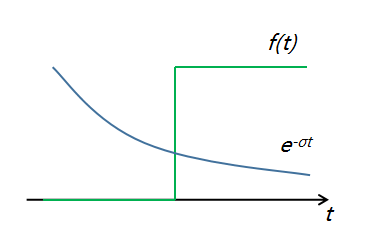
\includegraphics[scale=0.55]{LT思路.png}
\end{figure}
思路:$f(t)\cdot{e^{-\sigma{t}}}\cdot{U(t)}$满足Dirichlet条件后,可以对其进行FT。
\noindent
\begin{flalign*}\hspace{2em}
    F(\omega)&=\int_{\mathbb{R}}f(t)e^{-\sigma{t}}U(t)e^{-j\omega{t}}{\rm{d}}t &\\
    &=\int_{0}^{+\infty}f(t)e^{-(\sigma+j\omega)t}{\rm{d}}t &\\
    &\xlongequal{s=\sigma+j\omega}\int_{0}^{+\infty}f(t)e^{-st}{\rm{d}}t
\end{flalign*} \par
综上,LT定义:$F(s)=\int_{0}^{+\infty}f(t)e^{-st}{\rm{d}}t\quad$“单边LT”(无特殊说明,均默认为单边LT)

\subsection{逆变换定义}
$f(t)e^{-\sigma{t}}U(t)=\frac{1}{2\pi}\int_{\mathbb{R}}F(s)e^{-j\omega{t}}{\rm{d}}\omega$
\noindent
\begin{flalign*}\hspace{2em}
    f(t)&=\frac{1}{2\pi}\int_{\mathbb{R}}F(s)e^{-j\omega{t}}{\rm{d}}\omega\cdot{e^{\sigma{t}}}\cdot{U(t)} &\\
    &=\frac{1}{2\pi}\int_{\mathbb{R}}F(s)e^{(\sigma+j\omega)t}{\rm{d}}\omega\cdot{U(t)} &\\
    &\xlongequal{s=\sigma+j\omega}\frac{1}{2\pi}\int_{\mathbb{R}}F(s)e^{st}{\rm{d}}\omega\cdot{U(t)} &\\
    &\xlongequal{{\rm{d}}s=j{\rm{d}}\omega}\frac{1}{2\pi{j}}\int_{\mathbb{R}}F(s)e^{st}{\rm{d}}s\cdot{U(t)} &\\
    &\xlongequal{\omega\in(-\infty,+\infty)\rightarrow{s}\in(\sigma-j\infty,\sigma+j\infty)}\frac{1}{2\pi{j}}\int_{\sigma-j\infty}^{\sigma+j\infty}F(s)e^{st}{\rm{d}}s
\end{flalign*} \par
综上,逆变换定义:$f(t)=\frac{1}{2\pi{j}}\int_{\sigma-j\infty}^{\sigma+j\infty}F(s)e^{st}{\rm{d}}s$,$t\geqslant0$

\subsection{说明}
“s域”$\quad$“s domain” \par
$F(s)=\mathscr{L}\{f(t)\}$ $\quad$ $f(t)=\mathscr{L}^{-1}\{F(s)\}$

\section{LT$\quad$vs$\quad$FT}
相同:其本质依然是把信号分解为一系列正交函数集。\par
正交基:$\quad{e^{-st}=e^{-\sigma{t}}\cdot{e^{-j\omega{t}}}}\qquad$vs$\qquad{e^{-j\omega{t}}}$“$\approx$”$\int_{\mathbb{R}}e^{j\omega_1{t}}e^{-j\omega_2{t}}{\rm{d}}t=0$\par
\begin{figure}[h]
    \centering
    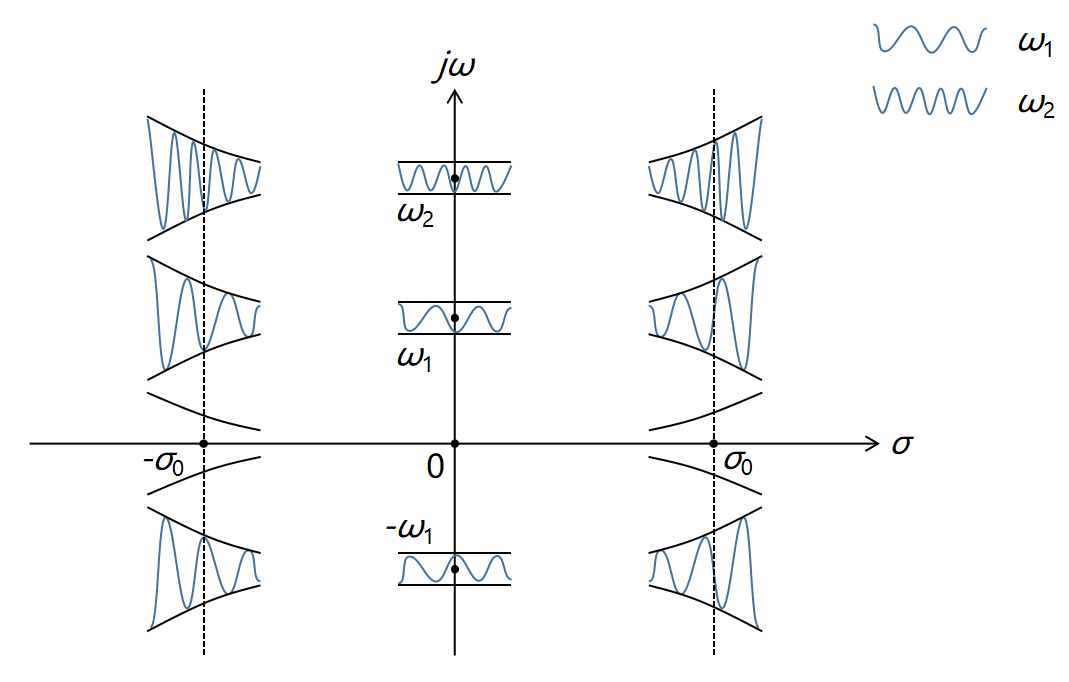
\includegraphics[scale=0.35]{LTvsFT.png}
\end{figure}
LT本质是FT的拓展,因此,两者应该性质相似、相通。

\newpage
\section{$F(\sigma,j\omega)$示意图}
\begin{figure}[h]
    \centering
    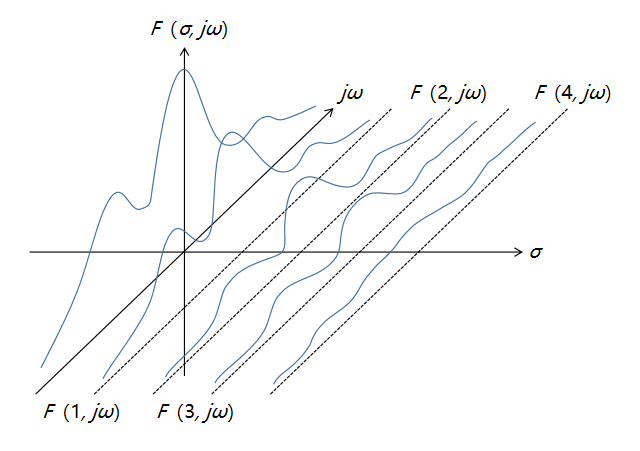
\includegraphics[scale=0.7]{F示意图.png}
\end{figure}

\section{收敛域}
例:$f(t)=e^{2t}\cdot{e^{-\sigma{t}}}\cdot{U(t)}\qquad$只有当$\sigma>2$时,LT“才有意义”。\par
$\lim_{t\rightarrow{+\infty}}f(t)e^{-\sigma{t}}=0$,所有满足上述条件的$\sigma>\sigma_0$称之为收敛域。
\begin{figure}[h]
      \centering
      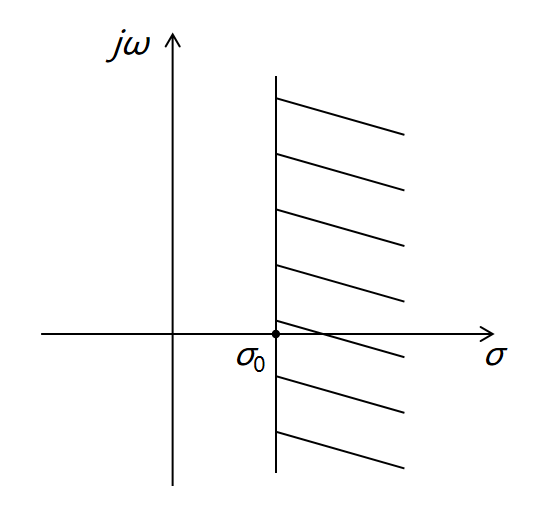
\includegraphics[scale=0.35]{收敛域.png}
\end{figure}
\begin{enumerate}[label=(\arabic*),itemindent=0pt,labelindent=\parindent,labelwidth=2em,labelsep=5pt,leftmargin=*]
      \item 收敛域一定是向“右边”扩展。
      \item 收敛域边界是垂直于$\sigma$轴的直线。
\end{enumerate}\par

\newpage
\section{FT与LT之间的联系}
\begin{figure}[h]
      \centering
      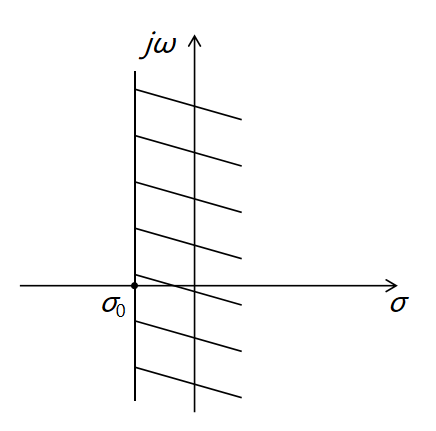
\includegraphics[scale=0.42]{LT与FT之间联系.png}
\end{figure}
\begin{enumerate}[label=(\arabic*),itemindent=0pt,labelindent=\parindent,labelwidth=2em,labelsep=5pt,leftmargin=*]
      \item 当$\sigma_0<0$时,$F(\omega)=F(s)\big{|}_{\sigma=0}$
      \item 当$\sigma_0>0$时,$F(\omega)$不存在
      \item 当$\sigma_0=0$时,$F(\omega)=\lim_{\sigma\rightarrow0}F(s)\equiv$广义FT
\end{enumerate}\par
综上,只有当$\sigma>\sigma_0$时,$F(s)$才有数值解。

\section{LT求解的例题}
\begin{enumerate}[label=(\arabic*),itemindent=0pt,labelindent=\parindent,labelwidth=2em,labelsep=5pt,leftmargin=*]
    \item $f(t)=e^{-\alpha{t}}$,$\alpha>0$ \par
          \noindent
          \begin{flalign*}
            F(s)&=\int_{0}^{+\infty}e^{-\alpha{t}}e^{-st}{\rm{d}}t &\\
            &=\int_{0}^{+\infty}e^{-(\alpha+s)t}{\rm{d}}t &\\
            &=\frac{1}{s+\alpha}
          \end{flalign*}
          因此,$e^{-\alpha{t}}\stackrel{\mathscr{L}}{\rightleftharpoons}\frac{1}{s+\alpha}$ \par
          $F(\omega)=\frac{1}{s+\alpha}\big{|}_{\alpha=0}=\frac{1}{\sigma+j\omega}$
    \item $f(t)=U(t)$ \par
          $F(s)=\frac{1}{s}$
          \noindent
          \begin{flalign*}
            F(\omega)&=\lim_{\sigma\rightarrow0}\frac{1}{s} &\\
            &=\lim_{\sigma\rightarrow0}\frac{1}{\sigma+j\omega} &\\
            &=\lim_{\sigma\rightarrow0}\frac{\sigma-j\omega}{\sigma^2+\omega^2} &\\
            &=\lim_{\sigma\rightarrow0}\frac{\sigma}{\sigma^2+\omega^2}-\lim_{\sigma\rightarrow0}\frac{j\omega}{\sigma^2+\omega^2} &\\
            &=\pi\delta(\omega)+\frac{1}{j\omega}
          \end{flalign*}
\end{enumerate}\par

\section{几种常见的LT}
\begin{tabular}{ c c c }
    时域 & $\quad$ & s域  \\
    $\delta(t)$ & $\quad$ & $1$ \\
    $U(t)$ & $\quad$ & $\frac{1}{s}$ \\
    $1$ & $\quad$ & $\frac{1}{s}$ \\
    $e^{\alpha{t}}$ & $\quad$ & $\frac{1}{s-\alpha}$ \\
    $\sin(\omega_0t)$ & $\quad$ & $\frac{\omega_0}{s^2+\omega_0^2}$ \\
    $\cos(\omega_0t)$ & $\quad$ & $\frac{s}{s^2+\omega_0^2}$ \\
    $\sum_{n=0}^{+\infty}f_0(t-nT_s)$ & $\quad$ & $\frac{1}{1-e^{-sT}}\int_{0}^{T}f_0(t)e^{-st}{\rm{d}}t=\frac{1}{1-e^{-sT}}F_0(s)$ \\
    $\sum_{n=0}^{+\infty}\delta(t-nT_s)$ & $\quad$ & $\frac{1}{1-e^{-sT}}$ \\
\end{tabular} \par

\end{document}